\documentclass[rgb]{beamer}

\usepackage[english]{babel}
\usepackage[utf8]{inputenc}
\usepackage{xcolor}
\usepackage{listings}
\usepackage{adjustbox}
\usepackage{amsmath}
\usepackage{multirow}
\usepackage[linewidth=1pt]{mdframed}

% Graphics
\usepackage{graphicx}

\usepackage{tikz}
\usetikzlibrary{calc,shapes.multipart,chains,arrows}

% Font
\usepackage{paratype}
\setbeamerfont{frametitle}{family=\bf}

% Beamer theme settings
\usecolortheme{seagull}
\setbeamertemplate{itemize item}{\raisebox{0.8mm}{\rule{1.8mm}{1.2mm}}}
\usenavigationsymbolstemplate{} % no navigation buttons

\usepackage{listings}

% Define Language
\lstdefinelanguage{fsharp}
{
  % list of keywords
  morekeywords={
    and,
    do,
    else,
    exception,
    for,
    fun,
    function,
    if,
    in,
    let,
    match,
    module,
    mutable,
    open,
    of,
    rec,
    then,
    try,
    type,
    unsafe,
    use,
    val,
    when,
    while,
    with,
  },
  sensitive=true, % keywords are not case-sensitive
  morecomment=[l]{//}, % l is for line comment
%  otherkeywords={>,<,=,<=,>=,!,*,/,-,+,|,&,||,&&,==,=>},
  morestring=[b]" % defines that strings are enclosed in double quotes
}

% Define Colors
\usepackage{color}
\definecolor{eclipseBlue}{RGB}{42,0.0,255}
\definecolor{eclipseGreen}{RGB}{63,127,95}
\definecolor{eclipsePurple}{RGB}{127,0,85}

\newcommand{\fop}[1]{\mbox{\ttfamily\color{eclipseBlue}#1}}
\newcommand{\fw}[1]{\mbox{\ttfamily\bfseries\color{eclipsePurple}#1}}

% Set Language
\lstset{
  language={fsharp},
  basicstyle=\ttfamily, % Global Code Style
  captionpos=b, % Position of the Caption (t for top, b for bottom)
  extendedchars=true, % Allows 256 instead of 128 ASCII characters
  tabsize=2, % number of spaces indented when discovering a tab
  columns=fixed, % make all characters equal width
  keepspaces=true, % does not ignore spaces to fit width, convert tabs to spaces
  showstringspaces=false, % lets spaces in strings appear as real spaces
  breaklines=true, % wrap lines if they don't fit
  frame=trbl, % draw a frame at the top, right, left and bottom of the listing
  frameround=tttt, % make the frame round at all four corners
  framesep=4pt, % quarter circle size of the round corners
  numbers=left, % show line numbers at the left
  numberstyle=\small\ttfamily, % style of the line numbers
  commentstyle=\slshape\bfseries\color{eclipseGreen}, % style of comments
  keywordstyle=\bfseries\color{eclipsePurple}, % style of keywords
  stringstyle=\color{eclipseBlue}, % style of strings
  emph=[1] {
    false,
    true,
    Set,
    Map,
    List,
    ImgUtil,
    Pegs,
    String,
    Array,
    Array2D
  },
  emphstyle=[1]{\color{eclipseBlue}},
  moredelim=**[is][\color{red}]{@@}{@@}
}

\newcommand{\theyear}{2020}
\newcommand{\sem}[1]{[\![#1]\!]}
\newcommand{\seme}[1]{\sem{#1}\varepsilon}
\newcommand{\semzero}[1]{\sem{#1}_0}

\newcommand{\emptymap}{\{\}}
\newcommand{\fracc}[2]{\begin{eqnarray} \frac{\begin{array}{c} #1
    \end{array}}{\begin{array}{c} #2 \end{array}} \end{eqnarray}}
\newcommand{\sembox}[1]{\hfill \normalfont \mbox{\fbox{\(#1\)}}}
\newcommand{\sempart}[2]{\subsubsection*{\rm\em #1 \sembox{#2}}}
\newcommand{\axiom}[1]{\begin{eqnarray} \begin{array}{c} #1 \end{array} \end{eqnarray}}
\newcommand{\fraccn}[2]{\refstepcounter{equation}\mbox{$\frac{\begin{array}{c} #1 \end{array}}{\begin{array}{c} #2 \end{array}}$}~(\arabic{equation})}
\newcommand{\fraccc}[2]{\mbox{$\frac{\begin{array}{c} #1 \end{array}}{\begin{array}{c} #2 \end{array}}$}}
\newcommand{\onepart}[1]{\noindent\hfill#1\hfill~\vspace{2mm}}
\newcommand{\twopart}[2]{\noindent\hfill#1\hfill#2\hfill~\vspace{2mm}}
\newcommand{\threepart}[3]{\noindent\hfill#1\hfill#2\hfill#3\hfill~\vspace{2mm}}
%\newcommand{\axiomm}[1]{\refstepcounter{equation}\mbox{$\begin{array}{c} #1 \end{array}$}~(\arabic{equation})}
\newcommand{\axiomm}[1]{$\begin{array}{c} #1 \end{array}$}
%\newcommand{\ar}[1]{\stackrel{#1}{\longrightarrow}}
\newcommand{\vd}{\vdash}
\newcommand{\Ran}{{\rm Ran}}
\newcommand{\Dom}{{\rm Dom}}
\newcommand{\kw}[1]{\texttt{#1}}
\newcommand{\id}[1]{\mbox{\it{#1}}}
\newcommand{\rarr}{\rightarrow}
\newcommand{\eval}{\rarr}
\newcommand{\evals}{\leadsto}
\newcommand{\larr}{\leftarrow}

\newcommand{\head}[1]{\vspace{3mm} \textbf{\normalsize #1}}
\newcommand{\headsp}[1]{\head{#1}\vspace{1ex}}
\newcommand{\size}{\ensuremath{\mathrm{size}}}
\renewcommand{\log}{\ensuremath{\mathrm{log}}}

\newcommand{\setallthemecolors}[1]{%
\setbeamercolor*{palette primary}{use=structure,fg=white,bg=#1}%
\setbeamercolor*{palette secondary}{use=structure,fg=white,bg=#1}%
\setbeamercolor*{palette tertiary}{use=structure,fg=white,bg=#1}}

\definecolor{black}{RGB}{0,0,0}
\definecolor{maroon}{RGB}{128,0,0}
\definecolor{olive}{RGB}{128,128,0}
\definecolor{green}{RGB}{0,128,0}
\definecolor{purple}{RGB}{128,0,128}
\definecolor{teal}{RGB}{0,128,128}
\definecolor{darkteal}{RGB}{0,92,92}
\definecolor{navy}{RGB}{0,0,128}
\definecolor{gray}{RGB}{128,128,128}
\definecolor{darkgray}{RGB}{60,60,60}
\definecolor{darkred}{RGB}{139,0,0}

%palette

% #173F5F (dark blue)
\definecolor{darkblue}{RGB}{23,63,95}
% #20639B (blue)
\definecolor{blue}{RGB}{32,99,155}
% #3CAEA3 (green)
\definecolor{magenta}{RGB}{60,174,163}
% #F6D55C (yellow)
\definecolor{yellow}{RGB}{246,213,92}
% #ED553B (red)
\definecolor{red}{RGB}{237,85,59}


\usecolortheme{whale}
\useoutertheme{infolines}
\useinnertheme{rectangles}

\newcommand{\popsettitle}[2]{%
\setallthemecolors{#1}%
\newcommand{\popemne}{#2}%
\title{Programmering og Problemløsning}%
\subtitle{#2}%
\author{Martin Elsman}%
\date{}%
\institute[DIKU]{Datalogisk Institut, Københavns Universitet (DIKU)}}

\newcommand{\popmaketitleframe}{%
  \frame{\titlepage%
   \vspace{-15mm}%
   \par\noindent\rule{\textwidth}{0.4pt}%

   \vspace{4mm}%
   \tableofcontents%
   \vspace{-4mm}%
   \par\noindent\rule{\textwidth}{0.4pt}%
  }%
  \section*{\popemne}%
}


\popsettitle{black}{Programmering med Lister og arrays (Recap)}

\begin{document}

\popmaketitleframe

%%%%%%%%%%%%%%%%%%%%%%%%%%%%%%%%%%%%%%%%%%%%%%%%
\subsection{Repræsentation af lister og arrays}
%%%%%%%%%%%%%%%%%%%%%%%%%%%%%%%%%%%%%%%%%%%%%%%%

\begin{frame}[fragile]
\begin{footnotesize}

  \head{Repræsentationen af lister}

  \begin{itemize}
  \item Syntax:
\begin{lstlisting}[numbers=none,frame=none]
let lst = [1; 2; 3; 4]
let lst2 = 5 :: List.tail (List.tail lst)
\end{lstlisting}

  \item Lagerrepræsentation:
    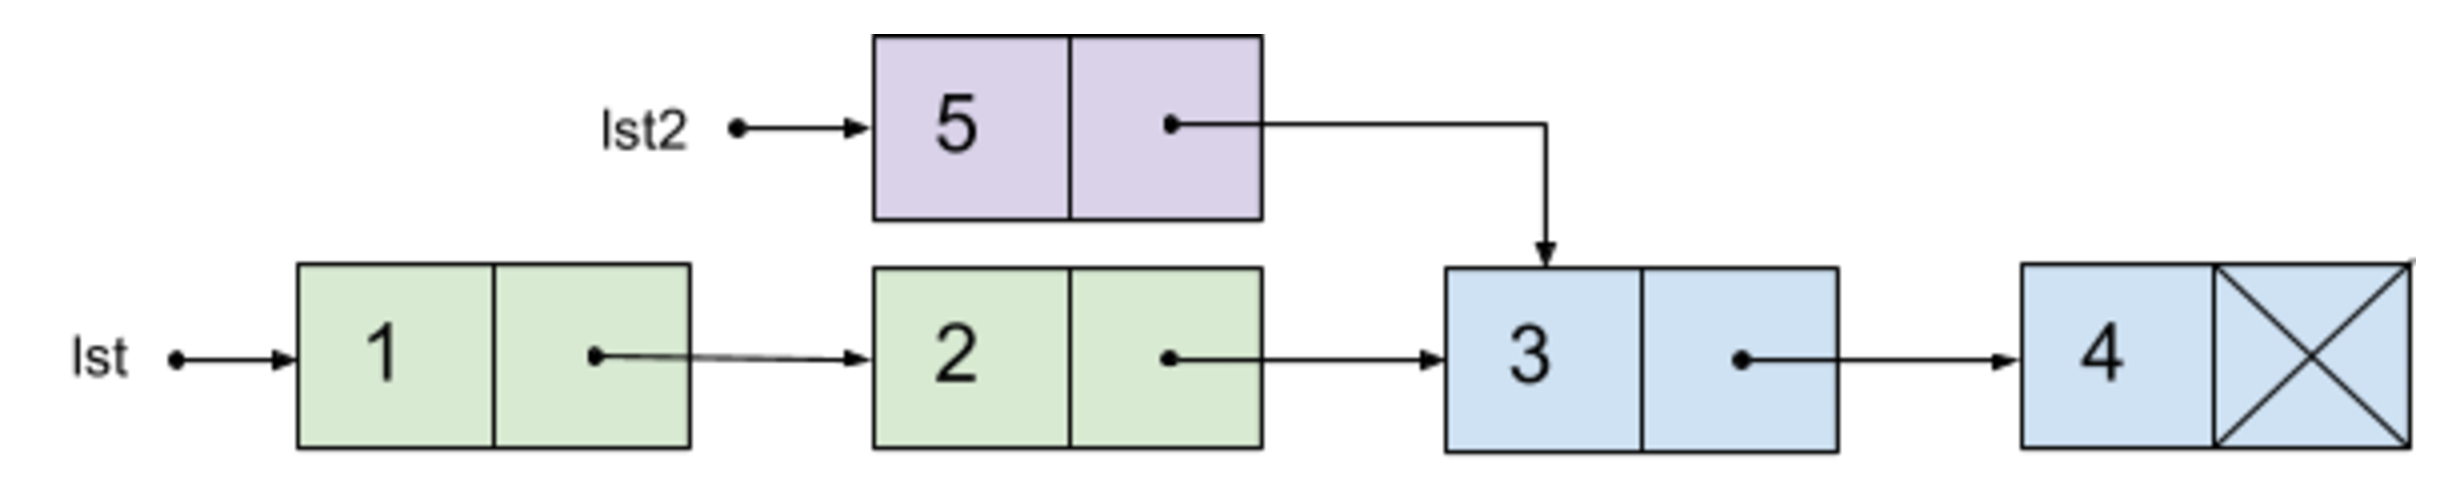
\includegraphics[width=0.9\textwidth]{list1234.png}

  \item Det er nemt at hægte et ekstra element på starten af en liste (\texttt{::}).

  \item Det er \textbf{IKKE} nemt (læs: hurtigt) at tilgå det sidste element i en liste.

  \item Lister er \emph{immutable}, dvs elementer kan ikke opdateres.

  \item Hvorfor kan immutabilitet være godt?
  \end{itemize}
\end{footnotesize}
\end{frame}

\begin{frame}[fragile]
\begin{footnotesize}
  \head{Repræsentationen af arrays}

  \begin{itemize}
  \item Syntax:
\begin{lstlisting}[numbers=none,frame=none]
let arr = [|1;2;3;4|]
\end{lstlisting}

  \item Lagerrepræsentation: \\
    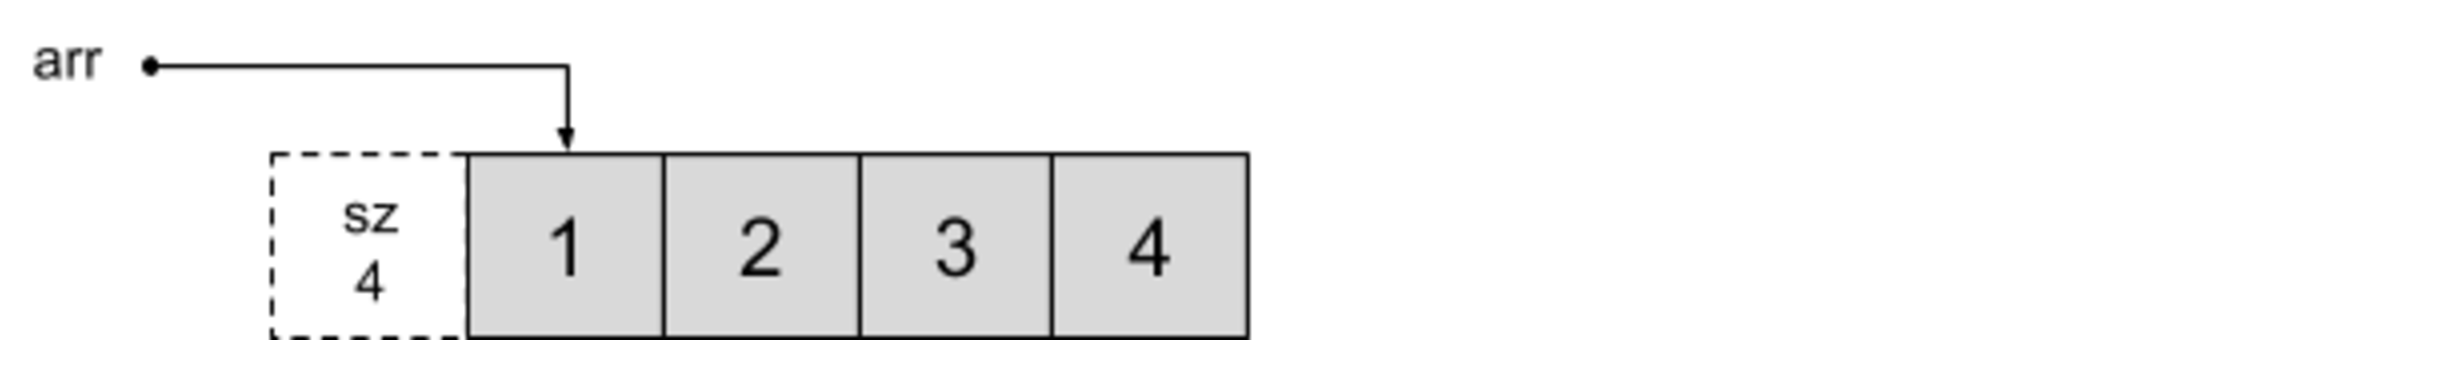
\includegraphics[width=0.9\textwidth]{array1234.png}
  \item Det er \textbf{IKKE} nemt at tilføje ekstra elementer.
  \item Det er nemt (hurtigt) at læse ethvert element i et array.

  \item Arrays er \emph{mutable}, dvs det er muligt (hurtigt) at
    opdatere ethvert element.
  \end{itemize}
\end{footnotesize}
\end{frame}


%%%%%%%%%%%%%%%%%%%%%%%%%%%%%%%%%%%%%%%%%%%%%%%%
\subsection{Imperativt gennemløb af lister}
%%%%%%%%%%%%%%%%%%%%%%%%%%%%%%%%%%%%%%%%%%%%%%%%

\begin{frame}[fragile]
\begin{footnotesize}

  \head{Imperativt gennemløb af lister}
  \vspace{1ex}

  Her er noget kode for en uheldig implementation af listesummation:
  \vspace{1ex}

\begin{lstlisting}[numbers=none,frame=none]
let lst = List.init 50000 (fun x -> x)         // BAD
let mutable i = 0                             // BAD
let mutable sum = 0                          // BAD
while (i < List.length lst) do              // BAD
  sum <- sum + lst.[i]                       // BAD
  i <- i + 1                                  // BAD
printf "%d\n" sum                              // BAD
\end{lstlisting}

\vspace{1ex}
\head{Tre problemer:}
\vspace{1ex}

  \begin{enumerate}
  \item \underline{\hspace{10cm}}  % kvadratisk runtime
  \item \underline{\hspace{10cm}}  % stor mulighed for fejl i indeksering <= ?
  \item \underline{\hspace{10cm}}  % mønster er ikke genbrugeligt
\end{enumerate}
\end{footnotesize}

\end{frame}


\begin{frame}[fragile]
\begin{footnotesize}

\head{Oversættelse og kørsel af \lstinline{bad_summation.fs}}

\begin{lstlisting}[numbers=none,frame=none]
// bad_summation.fs
let lst = List.init 50000 (fun x -> x)         // BAD
let mutable i = 0                             // BAD
let mutable sum = 0                          // BAD
while (i < List.length lst) do              // BAD
  sum <- sum + lst.[i]                       // BAD
  i <- i + 1                                  // BAD
printf "%d\n" sum                              // BAD
\end{lstlisting}

\head{Oversættelse og kørsel}

\begin{verbatim}
bash-3.2$ fsharpc --nologo bad_summation.fs
bash-3.2$ time mono bad_summation.exe
1249975000

real	0m8.112s
\end{verbatim}

\end{footnotesize}
\end{frame}

\begin{frame}[fragile]
\begin{footnotesize}
\head{Gennemløb af lister med \lstinline{for}-\lstinline{in}-\lstinline{do} konstruktionen}

\vspace{2ex}

Et bedre alternativ er at benytte den specielle \lstinline{for-in-do}
syntax til liste-gennemløb:

\vspace{1ex}

\begin{lstlisting}[numbers=none,frame=none,mathescape]
// better_summation.fs
let lst = List.init 50000 (fun x -> x)
let mutable sum = 0
for x in lst do sum <- sum + x
do printf "%d\n" sum
\end{lstlisting}

\vspace{1ex}

\head{Fordele:}
\begin{enumerate}
\item Ingen overhead ved liste-indicering eller kald til \lstinline{List.length}.
\item Simplere form for imperativ programmering; dog er \lstinline{sum} stadig mutable...
\end{enumerate}
\end{footnotesize}
\end{frame}

%%%%%%%%%%%%%%%%%%%%%%%%%%%%%%%%%%%%%%%%%%%%%%%%
\subsection{Modulet \lstinline{List}}
%%%%%%%%%%%%%%%%%%%%%%%%%%%%%%%%%%%%%%%%%%%%%%%%

\begin{frame}[fragile]
\begin{footnotesize}

\head{Modulet \lstinline{List}}

\vspace{1ex}

Modulet \lstinline{List} indeholder en lang række operationer på
lister.

\begin{lstlisting}[numbers=none]
// list creation
val init     : int -> (int -> 'a) -> 'a list

// list deconstruction
val head     : 'a list -> 'a
val tail     : 'a list -> 'a list

// list transformers
val map      : ('a -> 'b) -> 'a list -> 'b list
val map2     : ('a->'b->'c) -> 'a list -> 'b list -> 'c list
val filter   : ('a -> bool) -> 'a list -> 'a list

// list traversing
val length   : 'a list -> int   // length l = l.Length
val fold     : ('s -> 'a -> 's) -> 's -> 'a list -> 's
val foldBack : ('a -> 's -> 's) -> 'a list -> 's -> 's
val find     : ('a -> bool) -> 'a list -> 'a
...
\end{lstlisting}
\end{footnotesize}

\end{frame}

%%%%%%%%%%%%%%%%%%%%%%%%%%%%%%%%%%%%%%%%%%%%%%%%
\subsection{Intermezzo om funktionstyper og typevariabler}
%%%%%%%%%%%%%%%%%%%%%%%%%%%%%%%%%%%%%%%%%%%%%%%%

\begin{frame}[fragile]
\begin{footnotesize}

  \headsp{Funktionstyper}

  \vspace{2mm}
  \textbf{Q1:} Hvorfor beskæftiger vi os overhovedet med typer?
  \vspace{1mm}

  \begin{itemize}
  \item \underline{\hspace{10cm}}
  \end{itemize}

  \vspace{2mm}
  \textbf{Q2:} Hvad beskriver funktionstypen \lstinline{int->int}
  \vspace{1mm}

  \begin{itemize}
  \item \underline{\hspace{10cm}}
  \end{itemize}

  \vspace{2mm}
  \textbf{Q3:} I den kontekst, hvad er forskellen på værdiorienteret (funktionel) programmering og effektfuld (imperativ) programmering?
  \vspace{1mm}

  \begin{itemize}
  \item \underline{\hspace{10cm}}
  \end{itemize}

  \vspace{2mm}
  \textbf{Q4:} Beskriv forskellen på typerne \lstinline{int->int->int} og \lstinline{(int->int)->int}
  \vspace{1mm}

  \begin{itemize}
  \item \underline{\hspace{10cm}}
  \end{itemize}

  \vspace{2mm}
  \textbf{Q5:} Hvilken forskel kan der være på følgende to funktioner:
  \vspace{1mm}
\begin{lstlisting}[frame=none]
  val toDKK : string * float -> float   // toDDK ("USD",5.0)
  val toDKK : string -> float -> float  // toDKK "USD" 5.0
\end{lstlisting}

\end{footnotesize}
\end{frame}

\begin{frame}[fragile]
\begin{footnotesize}

  \headsp{Typevariabler}
  \vspace{2mm}

  Typevariabler (f.eks. \lstinline{'a} og \lstinline{'S}) benyttes til at skrive
  \emph{generiske} funktioner, som er funktioner der kan anvendes på
  værdier af forskellig type.

  \vspace{4mm}
  \textbf{Q1:} Hvad er typen for funktionen \lstinline{List.length}?
  \vspace{1mm}

  \begin{itemize}
  \item \underline{\hspace{10cm}}
  \end{itemize}

  \vspace{4mm}
  \textbf{Q2:} Hvad er typen for funktionen \lstinline{List.map}?
  \vspace{1mm}

  \begin{itemize}
  \item \underline{\hspace{10cm}}
  \end{itemize}

  \vspace{4mm} \textbf{Bemærk:} Det vil være besværligt hvis
  programmøren skal være eksplicit omkring typer alle steder i et
  program. Derfor har F\#
  \emph{typeinferens}, hvilket betyder at programmøren ofte kan
  udelade typeannoteringer.
\end{footnotesize}
\end{frame}


%%%%%%%%%%%%%%%%%%%%%%%%%%%%%%%%%%%%%%%%%%%%%%%%
\subsection{Dynamisk konstruktion af lister}
%%%%%%%%%%%%%%%%%%%%%%%%%%%%%%%%%%%%%%%%%%%%%%%%

\begin{frame}[fragile]
\begin{footnotesize}

  \head{Dynamisk konstruktion af lister}

  \vspace{1ex}

  Funktionen \lstinline{List.init} gør det muligt at opbygge en liste
  dynamisk fra bunden:

\begin{lstlisting}[numbers=none,frame=none,mathescape]
val init : int -> (int -> 'a) -> 'a list

 init $n$ f
   = [f $0$; f $1$; f $2$; ...; f $(n-1)$]
\end{lstlisting}

  \vspace{1ex}

  \head{Eksempel}

\begin{lstlisting}[numbers=none,frame=none,mathescape]
let sz = 2 + 3
let lst = List.init sz (fun x -> x * 2 + 1)

//  = [0*2+1; 1*2+1; 2*2+1; 3*2+1; 4*2+1]
// $\evals$  [1; 3; 5; 7; 9]
\end{lstlisting}

\end{footnotesize}
\end{frame}

%%%%%%%%%%%%%%%%%%%%%%%%%%%%%%%%%%%%%%%%%%%%%%%%
\subsection{Transformation af lister}
%%%%%%%%%%%%%%%%%%%%%%%%%%%%%%%%%%%%%%%%%%%%%%%%

\begin{frame}[fragile]
\begin{footnotesize}
  \head{Transformation af lister --- \lstinline{map}}
\vspace{0.5ex}

\begin{lstlisting}[numbers=none,frame=none,mathescape]
val map : ('a -> 'b) -> 'a list -> 'b list

 map f [v$_0$; v$_1$; v$_2$; ...; v$_n$]
   = [f v$_0$; f v$_1$; f v$_2$; ...; f v$_n$]
\end{lstlisting}

\head{Eksempel}
\vspace{0.5ex}
\begin{lstlisting}[numbers=none,frame=none,mathescape]
let vs = List.map (fun x -> x+1) [10; 20; 30]

//  = [10+1; 20+1; 30+1]  $\evals$  [11; 21; 31]
\end{lstlisting}

\end{footnotesize}
\end{frame}

%%%%%%%%%%%%%%%%%%%%%%%%%%%%%%%%%%%%%%%%%%%%%%%%
\subsection{Gennemløb af lister med \lstinline{fold}}
%%%%%%%%%%%%%%%%%%%%%%%%%%%%%%%%%%%%%%%%%%%%%%%%

\begin{frame}[fragile]
\begin{footnotesize}

  \head{Listefoldninger --- \lstinline{fold}}

  \vspace{1ex}

  Listefoldninger er generiske funktioner der gør det muligt at
  gennemløbe en liste for samtidig at foretage beregninger på
  elementerne, f.eks. for at opbygge en ny datastruktur.

  \vspace{1ex}

\begin{lstlisting}[numbers=none,frame=none,mathescape]
val fold     : ('a -> 'b -> 'a) -> 'a -> 'b list -> 'a

 fold f a [x$_0$;x$_1$;x$_2$;...;x$_n$]
   = f ... (f (f (f a x$_0$) x$_1$) x$_2$) ... x$_n$
\end{lstlisting}

\headsp{Husk:}
\begin{itemize}
\item En funktion kaldes først når argumenterne er evalueret til værdier!
\item Dette princip kaldes ``Call-by-value''.
\end{itemize}

\end{footnotesize}
\end{frame}

\begin{frame}[fragile]
\begin{footnotesize}

\head{Eksempel: Summation af elementerne i en liste}
\vspace{1ex}

\begin{lstlisting}[numbers=none,frame=none,mathescape]
let sum = List.fold (+) 0 [3;6;2;5]

//   = (((0 + 3) + 6) + 2) + 5
// $\eval$ ((3 + 6) + 2) + 5
// $\eval$ (9 + 2) + 5  $\eval$  11 + 5  $\eval$  16
\end{lstlisting}

\vspace{1ex}
\head{Eksempel: Find det mindste element i en liste}
\vspace{1ex}

\begin{lstlisting}[numbers=none,frame=none,mathescape]
let min x y = if x < y then x else y
let maxInt = System.Int32.MaxValue  // = 2147483647
let min_elem = List.fold min maxInt [3;6;2;5]

//   = min (min (min (min 2147483647 3) 6) 2) 5
// $\eval$ min (min (min 3 6) 2) 5
// $\eval$ min (min 3 2) 5  $\eval$  min 2 5  $\eval$  2
\end{lstlisting}

\end{footnotesize}
\end{frame}

\begin{frame}[fragile]
\begin{footnotesize}
  \head{Eksempel: Reverser en liste}
\vspace{1ex}

\begin{lstlisting}[numbers=none,frame=none,mathescape]
let f a x = x :: a
let rev xs = List.fold f [] xs

let ex = rev [1;2;3]

// = f (f (f [] 1) 2) 3
// $\eval$ f (f (1 :: []) 2) 3  $\eval$  f (2 :: 1 :: []) 3
// $\eval$ 3 :: 2 :: 1 :: []
\end{lstlisting}

\end{footnotesize}
\end{frame}

\subsection*{Konklusion}
\begin{frame}[fragile]
  \headsp{Konklusion}

  \vspace{3mm}
  \tableofcontents
\end{frame}

\end{document}
